\section{Sympathy for the Devil}

\begin{quotex}
I will no longer talk much with you, for the ruler of this world is coming. He has no power over me.
\flright{\textsc{John 14:30}}
\end{quotex}


\paragraph{Council of Evil}

\begin{wrapfigure}{rt}{.3\textwidth}
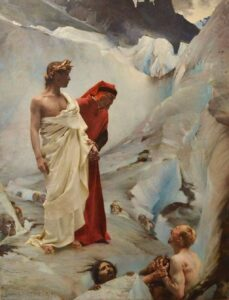
\includegraphics[width=.25\textwidth]{DanteVirgil_Gustave_Courtois-229x300.jpg}
\end{wrapfigure}

\textbf{Mary of Agreda} had a vision of the coming of the Prince of this World. The world is depraved, that is, good and evil are not easily separated. Science is concerned with events that are immediately verifiable. Humans seldom think further than a five or ten year plan. However, the Prince plans over the course of centuries, longer than what science can process. People act from motives and reasons of which they are seldom fully conscious. Their views of world events are no deeper than a script for a Batman movie, replete with good guys and evil villains. Solange Hertz describes Mary's vision:

\begin{quotex}
Whoever thinks history ``just happens'' needs to read the \emph{Mystical City of God} for proper perspective. Called on for their opinions after the Crucifixion, the higher ranking demons agreed that it would be impossible to reverse the Redemption now accomplished by Christ, but they could labor to prevent the application of its fruits. They advised that, ``in accordance with the new order of assistance and favor established by God for the salvation of men, they should seek new ways of hindering and preventing the work of God by deceits and temptations so much the greater.'' Sinful men's lives are too short, their wills too weak, their thinking too limited. Bound to bodies shackled by recurring hunger and fatigue, they are incapable of an effort which must be sustained at white heat literally through centuries.
\flright{\textsc{Solange Hertz}}
\end{quotex}


\paragraph{Lust for Power}


\begin{quotex}
The devil took him to a very high mountain, and showed him all the kingdoms of the world and their glory; and he said to him: All these I will give you, if you will fall down and worship me. Then Jesus said to him: Begone, Satan! for it is written, ``You shall worship the Lord your God and him only shall you serve.''
\flright{\textsc{Matthew 4:8--10}}
\end{quotex}


This third temptation in the desert was resisted by Christ, but is too tempting for most in power today. The secret power of the temptation is that it denies that God is the creator. The corollary is that man is the creator of the world. Just as the Logos speaks the world into existence, man tries to create his own world by the redefinition of words.

\paragraph{Virgil and Dante}

Note this painting of Virgil and Dante visiting hell by Gustav Courtois. It shows two contrasting attitudes toward the evil in the world. Virgil shows a Stoic detachment while Dante is holding onto Virgil for dear life. Unlike Virgil, he shows interest in their suffering.

\paragraph{Death and Immortality}


Vladimir Soloyvov appeared on the world stage at the end of the 19\textsuperscript{th} century as a new beacon. He was not understood, and his thought is still being digested. As we mentioned last time, the Common Task inaugurated by Nikolai Fyodorov, was his starting point. Death is the ineradicable evil in the world. However, Fyodorov's proposed solution of a physical, medical resurrection of the dead is untenable. What is the point, Solovyov asks, is bring the dead back into the world of evil?

There is no war of the good against the evil; they cannot be so easily separated. Rather the world itself is evil and is in need of salvation. The opposite of death is immortality, specifically, immortality in Christ. Just as the telos of animals (he wrote to Tolstoy) is rationality, immortality is the telos of humankind. This will be spearheaded by a higher order of evolved Christians. They will create intentional communities of spirit based not on blood, nation, or family ties, but on spiritual development.

A divine-human interactivity provides the motor forces. He identifies them as godmanhood, Christ the Logos, Sophia the World Soul. Godmanhood is the divinization of the human being, Christ is the uplifting force, and Sophia is active in the world, the opponent of the Prince of the World, envisioned as stomping on the serpent.

\paragraph{Evil in the World}


\begin{quotex}
We Christians should search our consciences and see whether we do not tend to pay too little attention to the spiritual powers of genuine mysticism and so let many people of real spiritual depth drift away from us. That is something which we should always bear in mind, even while rejecting, as we must necessarily do, the whole movement as it presents itself to us today.
\flright{\textsc{Fr. Alois Wiesinger}, \emph{Occult Phenomena}\footnote{\url{https://www.gornahoor.net/library/occultPhenomena.pdf}}}
\end{quotex}


Fr. Alois Wiesinger was speaking of Rudolf Steiner, who appeared at a time of cultural decline to adapt spiritual knowledge to the modern age. But there are two Steiners. The first is Steiner the philosopher and metaphysician who writes often lucidly on those topics. The second Steiner is prone to dreamy, fantasies, which he described as ``Spiritual Science''. However, his close student, Valentin Tomberg, came to the realization that it could not be a science because his visions were neither verifiable not repeatable. To Steiner's credit, he recognized the significance of Solovyov long before Western academicians. Hence, I will simply quote from the essay previously mentioned. The significance of resurrection for Solovyov is made totally clear.

\begin{quotationx}
His idea is this: There is evil in the world, wickedness in the world. If we, with our senses, behold the evil and wickedness, we cannot deny that the world is full of both. This, says Soloviev, refutes the divinity of the world, for when we behold the world with our senses, how can we believe in a divine world, since a divine world can certainly not exhibit evil! But the senses perceive evil everywhere and the extreme evil is death. Because death is in the world, the world is revealed in all its evil and wickedness. The arch-evil is death!

Look at the world with your ordinary senses; try to understand the world with your ordinary mind. You can never deny the existence of evil in the world, and to desire to understand death would be absurd! Death exists. Knowledge acquired through the senses reveals a world of wickedness, a world of evil. Can we believe, asks Soloviev, that this world is divine when it shows us that it is full of evil, when it shows us death at every step? Nevermore can we believe that a world that shows us death is a divine world. For in God there can be no evil, no wickedness, above all, not the arch-evil death. In God there cannot be death.

If, therefore, God were to come into the world, if God were to appear, should we be able immediately to believe him to be God? No, we should not! He would have to establish his identity first. If a being claiming to be God were to appear, we should not believe him. He would have to prove his identity by producing something of the nature of a world document that would enable us to recognize him as God! Nothing of the kind exists in the world. God cannot prove his identity through what is in the world, for everything in the world contradicts the divine nature. By what means, then, can he prove his identity? Only by showing, when he comes into the world, that he has conquered death, that death can have no power over him. We should never believe Christ to be God if He did not prove his identity. But Christ did so, inasmuch as He has risen, inasmuch as He has shown that the arch-evil, death, is not in Him.

It is a consciousness of the divine that is based solely upon the actual, historical resurrection of Christ, Who, as God, proves His identity. Soloviev goes on to say: Nothing in the world, with the single exception of the Resurrection, enables us to realize that a God exists. If Christ had not risen, all our belief would be vain, and everything we could say about a divine nature in the world, this too would be vain. Soloviev quotes these words of St. Paul again and again.

If we look at the world, we see therein only evil, wickedness, degeneration, senselessness. If Christ had not risen, the world would be meaningless, therefore Christ has risen! Note this sentence well, for it is a cardinal saying of one of the greatest thinkers of Eastern Europe: ``If Christ had not risen the world would be senseless, therefore Christ has risen.'' Soloviev has said: ``There may be people who think it illogical when I say, if Christ had not risen the world would be senseless; therefore, Christ has risen --- but this is far better logic than any you can adduce against me.''
\end{quotationx}

\url{https://www.youtube.com/watch?v=GgnClrx8N2k} 

\flrightit{Posted on 2022-03-17 by Cologero}

\begin{center}* * *\end{center}

\begin{footnotesize}
\begin{sffamily}
\texttt{Auld Wat on 2022-03-18 at 05:40 said:}

I finished a Canticle for Leibowitz yesterday. The last abbot of the order is talking with an atheist doctor who just wants to ease the pain of his patients through euthanasian, he admonishes him thus ``you are a soul, you only temporarily have a body.'' A helpful reminder which chimes with traditional Catholic teaching as in the daily prayer, ``Remember, Christian soul, that thou has this day, and every day of thy life ... a body to mortify and a soul to save''.

There's no surprise that Our Lady called on us to repent of our sins at Fatima, and that in the last two destructive centuries two long held beliefs of her greatness became dogmas. The world might not see it but Sophia is moving behind the scenes in parallel to Satan, captured brilliantly at the beginning of the scene where Christ carries the Cross to Golgotha in the Passion of the Christ.

\hfill

\texttt{Oswald Spengler on 2022-03-18 at 22:11 said:}

If you're going to post the Rolling Stones, I'm surprised you didn't give a nod to Mikhail Bulgakov whose novel inspired that song. Bulgakov was very much in the Russian spiritual continuum descending from Soloviev

\hfill

\texttt{Cologero on 2022-03-18 at 22:18 said:}

You are confusing Mikhail Bulgakov with Sergei Bulgakov. That is not an uncommon mistake.

\hfill

\texttt{Balder on 2022-03-19 at 04:13 said:}

That RS song is really bad.

In the Bulgakov novel Satan merely gives men what they desire the most, ergo, he has an educational function for the souls of man. A late Finnish esoterist Pekka Ervast said that the angel Satan has as his kingdom the planet earth and in his function as the prince of the world he cannot do otherwise than give man his powers, knowing at the same time fully well that they misuse it for selfish ends. At the same time he said that we as humans are incapable of understanding such holiness and this is why men throw their own faults in his shoulders, and that Satan is always ``happy'' when men don't fall for his temptations and overcome themselves, and after Christ came the scepter of Satan (Justice/Rigor) is being slowly but steadily given into the hands of Christ (Love/Mercy). I guess this is more in line with a theosophical conception of Satan and goes against the grain of Christian theological thought where his function is that of an evil anti-god. But the same line of thought can also be seen in an esoteric interpretation of Job, for example.

\hfill

\texttt{Balder on 2022-03-27 at 18:55 said:}

Perhaps the mystery of Satan can be explained in kabbalistic terms by the bright and obscure faces of Metatron aka Satan in this picture would be the ``fallen Metatron'', so like unto Him that man does not recognize his bright face until he knows himself?

\hfill

\texttt{Balder on 2022-03-27 at 19:05 said:}

Just as God is surrounded by the ``cloud of unknowing'', the holy darkness, so is Satan surrounded by the ``unholy darkness'', the deeds of evil in which man projects the ``devil'' that is in reality only his own working.

\hfill

\texttt{Taivasvaeltaja on 2023-10-28 at 13:56 said:}

``I have never understood men don't appreciate civilized table conversation and the Company of beautiful women.''

-- Master Woland

\end{sffamily}
\end{footnotesize}

